% Author: Izaak Neutelings (October 2020)
% https://mathworld.wolfram.com/PhasePortrait.html
\documentclass[border=3pt,tikz]{standalone}
\usepackage{amsmath} % for \dfrac
\usepackage{physics,siunitx}
\usepackage{tikz,pgfplots}
\usepackage[outline]{contour} % glow around text
\contourlength{1.0pt}
\usetikzlibrary{angles,quotes} % for pic (angle labels)
\usetikzlibrary{arrows.meta}
\usetikzlibrary{decorations.markings}
%\usetikzlibrary{bending} % for arrow head angle
\tikzset{>=latex} % for LaTeX arrow head
\usepackage{xcolor}

\colorlet{xcol}{blue!60!black}
\colorlet{myred}{red!80!black}
\colorlet{myblue}{blue!80!black}
\colorlet{mygreen}{green!40!black}
\colorlet{myorange}{orange!90!black}
\colorlet{mypurple}{red!50!blue!90!black!80}
\colorlet{mydarkred}{myred!80!black}
\colorlet{mydarkblue}{myblue!80!black}
\tikzstyle{xline}=[xcol,thick]
\tikzstyle{width}=[{Latex[length=5,width=3]}-{Latex[length=5,width=3]},thick]
\tikzset{
  traj/.style 2 args={xline,postaction={decorate},decoration={markings,
    mark=at position #1 with {\arrow{<}},
    mark=at position #2 with {\arrow{<}}}
  }
}
\def\tick#1#2{\draw[thick] (#1)++(#2:0.12) --++ (#2-180:0.24)}
\def\N{100} % number of samples


\begin{document}


% CIRCLE on axis
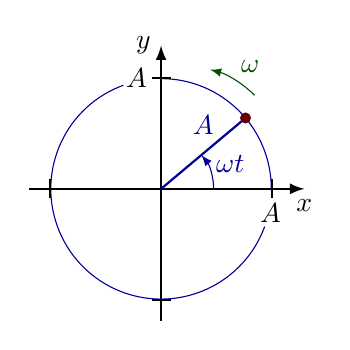
\begin{tikzpicture}
  \def\A{1.4}
  \def\ang{40}
  \coordinate (O) at (0,0);
  \coordinate (X) at (\A,0);
  \coordinate (R) at (\ang:\A);
  \draw[->,thick] (-1.2*\A,0) -- (1.3*\A,0) node[below] {$x$};
  \draw[->,thick] (0,-1.2*\A) -- (0,1.3*\A) node[left] {$y$};
  \node[inner sep=2] (R') at (R) {};
  \draw[xcol] (0:\A) arc(0:90:\A);
  \draw[xcol] (110:\A) arc(110:340:\A);
  \draw[xcol,thick,line cap=round] (O) -- (R) node[midway,above=3] {$A$};
  \tick{0,-\A-0.008}{0}; %node[left=-1,scale=1] {$A$};
  \tick{0, \A+0.008}{0} node[left=-2,scale=1] {$A$};
  \tick{-\A-0.008,0}{90}; %node[below=-1,scale=1] {$A$};
  \tick{ \A+0.008,0}{90} node[left=0.5,below=-2,scale=1] {$A$};
  \draw pic[->,"$\omega t$",xcol,draw=xcol,angle radius=19,angle eccentricity=1.4] {angle=X--O--R};
  \fill[myred!50!black] (R) circle (0.07);
  \draw[->,mygreen!80!black] (\ang+5:1.2*\A) arc(\ang+5:\ang+35:0.9*\A) node[midway,above right=-1] {$\omega$};
\end{tikzpicture}


% CIRCLE on axis + phase
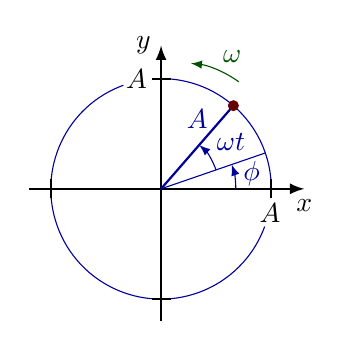
\begin{tikzpicture}
  \def\A{1.4}
  \def\ang{30}
  \def\phase{19}
  \coordinate (O) at (0,0);
  \coordinate (X) at (\A,0);
  \coordinate (R0) at (\phase:\A);
  \coordinate (R) at (\ang+\phase:\A);
  \draw[->,thick] (-1.2*\A,0) -- (1.3*\A,0) node[below] {$x$};
  \draw[->,thick] (0,-1.2*\A) -- (0,1.3*\A) node[left] {$y$};
  \node[inner sep=2] (R') at (R) {};
  \draw[xcol] (0:\A) arc(0:90:\A);
  \draw[xcol] (110:\A) arc(110:340:\A);
  \draw[xcol,thick,line cap=round] (O) -- (R) node[midway,above=3] {$A$};
  \draw[xcol,thin] (O) -- (R0);
  \tick{0,-\A}{0}; %node[left=-1,scale=1] {$A$};
  \tick{0, \A}{0} node[left=-2,scale=1] {$A$};
  \tick{-\A,0}{90}; %node[below=-1,scale=1] {$A$};
  \tick{ \A,0}{90} node[left=0.5,below=-2,scale=1] {$A$};
  \draw pic[->,"$\phi$",xcol,draw=xcol,angle radius=27,angle eccentricity=1.23] {angle=X--O--R0};
  \draw pic[->,"$\omega t$",xcol,draw=xcol,angle radius=21,angle eccentricity=1.45] {angle=R0--O--R};
  \fill[myred!50!black] (R) circle (0.07);
  \draw[->,mygreen!80!black] (\ang+\phase+5:1.2*\A) arc(\ang+\phase+5:\ang+\phase+35:0.9*\A) node[midway,above right=-1] {$\omega$};
\end{tikzpicture}


% COS
\def\xmax{6.6} % max x axis
\def\ymax{1.2} % max y axis
\def\A{0.8}    % amplitude
\def\om{(2.55*360/(0.94*\xmax))} % angular frequency in degrees
\begin{tikzpicture}
  
  % AXIS
  \draw[->,thick] (0,-\ymax) -- (0,\ymax) node[left,xcol] {$x$};
  \draw[->,thick] (-0.2*\ymax,0) -- (\xmax,0) node[below] {$t$};
  \draw[dashed] ({360/\om},1.2*\A) --++ (0,-2.7*\A);
  \tick{0,\A}{0} node[left=-1,scale=0.9] {$A$};
  \tick{{360/\om},0}{90} node[below,scale=0.9] {\contour{white}{$T$}};
  \tick{{720/\om},0}{90} node[below,scale=0.9] {$2T$};
  \draw[<->]
    (0,-1.35*\A) --++ ({360/\om},0)
    node[midway,fill=white,inner sep=1,scale=0.9] {$T = 2\pi/\omega$};
  
  % PLOT
  \draw[xline,samples=\N,smooth,variable=\x,domain=0:0.94*\xmax]
    plot(\x,{\A*cos(\om*\x)});
  %\node[xcol,above=2,right=4] at ({720/\om},\A) {$x(t)=A\cos(\omega t)$};
  
\end{tikzpicture}


% COS - phase
\begin{tikzpicture}
  \def\phase{60}
  
  % AXIS
  \draw[->,thick] (0,-\ymax) -- (0,\ymax) node[left,xcol] {$x$};
  \draw[->,thick] (-0.2*\ymax,0) -- (\xmax,0) node[below] {$t$};
  \tick{0,\A}{0} node[left=-1,scale=0.9] {$A$};
  \tick{{\phase/\om},0}{90} node[below,scale=0.9] {$t_0$};
  \draw[dashed] ({\phase/\om},0) --++ (0,1.2*\A);
  \draw[dashed] ({180/\om},-1.3*\A) --++ (0,1.5*\A);
  \draw[dashed] ({(180+\phase)/\om},-1.3*\A) --++ (0,1.5*\A);
  \draw[->]
    ({180/\om},-1.25*\A) --++ ({\phase/\om},0)
    node[midway,below,scale=0.9] {$t_0 = \phi/\omega$};
  
  % PLOT
  \draw[xcol!30,thin,dashed,samples=\N,smooth,variable=\x,domain=0:0.94*\xmax]
    plot(\x,{\A*cos(\om*\x)});
  \draw[xline,samples=\N,smooth,variable=\x,domain=0:0.94*\xmax]
    plot(\x,{\A*cos(\om*\x-\phase)});
  \tick{{(360+\phase)/\om},0}{90} node[below,scale=0.9] {\contour{white}{$t_0+T$}};
  \tick{{(720+\phase)/\om},0}{90} node[below,scale=0.9] {\contour{white}{$t_0+2T$}};
  
\end{tikzpicture}


% COS - phase - vertical shift
\begin{tikzpicture}
  \def\phase{60}
  \def\C{0.5*\A}
  
  % AXIS
  \draw[->,thick] (0,\C-\ymax) -- (0,\C+1.05*\ymax) node[left,xcol] {$y$};
  \draw[->,thick] (-0.2*\ymax,0) -- (\xmax,0) node[below] {$t$};
  \tick{0,\C+\A}{0} node[left=-1,scale=0.9] {$A+y_0$};
  \tick{0,\C-\A}{0} node[left=-1,scale=0.9] {$-A+y_0$};
  \tick{0,\C}{0} node[left=-1,scale=0.9] {$y_0$};
  
  % PLOT
  \draw[dashed] (0,\C) --++ (0.95*\xmax,0);
  \draw[xline,samples=\N,smooth,variable=\x,domain=0:0.94*\xmax]
    plot(\x,{\C+\A*cos(\om*\x-\phase)});
  %\tick{{(360+\phase)/\om},0}{90} node[below,scale=0.9] {\contour{white}{$t_0+T$}};
  %\tick{{(720+\phase)/\om},0}{90} node[below,scale=0.9] {\contour{white}{$t_0+2T$}};
  
\end{tikzpicture}


% COS - damped
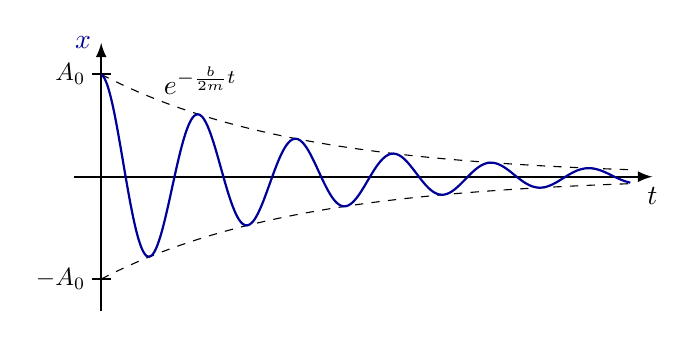
\begin{tikzpicture}
  \def\xmax{7.0} % max x axis
  \def\ymax{1.7}
  \def\A{1.3}
  \def\om{(5.3*360/(0.94*\xmax))}
  \def\t{1800/(0.94*\xmax)}
  \def\T{2.5}
  
  % AXIS
  \draw[->,thick] (0,-\ymax) -- (0,\ymax) node[left,xcol] {$x$};
  \draw[->,thick] (-0.2*\ymax,0) -- (\xmax,0) node[below] {$t$};
  \tick{0,\A}{0} node[left=-1,scale=0.9] {$A_0$};
  \tick{0,-\A}{0} node[left=-1,scale=0.9] {$-A_0$};
  
  % PLOT
  \draw[dashed,samples=\N,smooth,variable=\t,domain=0:0.96*\xmax]
    plot(\t,{\A*exp(-\t/\T)}) plot(\t,{-\A*exp(-\t/\T)});
  \draw[xline,samples=100+\N,smooth,variable=\t,domain=0:0.96*\xmax]
    plot(\t,{\A*exp(-\t/\T)*cos(\om*\t)});
  \node[above=4] at (0.18*\xmax,{\A*exp(-0.18*\xmax/\T)}) {$e^{-\frac{b}{2m}t}$};
  
\end{tikzpicture}


% COS - overdamped
% https://en.wikipedia.org/wiki/Harmonic_oscillator#Universal_oscillator_equation
% https://brilliant.org/wiki/damped-harmonic-oscillators/
% https://beltoforion.de/en/harmonic_oscillator/
% http://hyperphysics.phy-astr.gsu.edu/hbase/oscda.html#c1
% http://hyperphysics.phy-astr.gsu.edu/hbase/oscda2.html#c1
% https://ocw.mit.edu/courses/mathematics/18-03sc-differential-equations-fall-2011/unit-ii-second-order-constant-coefficient-linear-equations/damped-harmonic-oscillators/MIT18_03SCF11_s13_2text.pdf
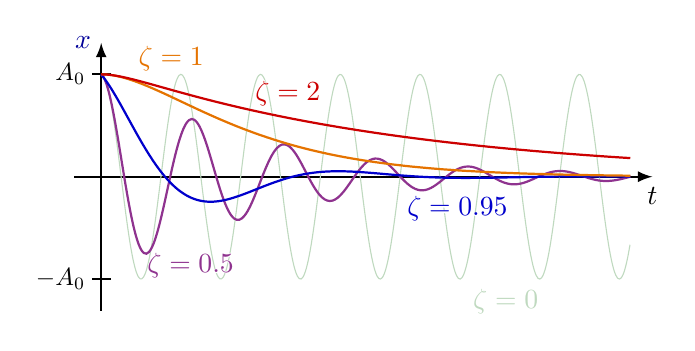
\begin{tikzpicture}
  \def\xmax{7.0} % max x axis
  \def\ymax{1.7} % max y axis
  \def\A{1.3}
  \def\om{(6.5/(0.94*\xmax))} % natural omega_0
  \def\Za{0.50} % zeta underdamped 1
  \def\Zb{0.95} % zeta underdamped 2
  \def\Zc{1.00} % zeta critically damped
  \def\Zd{2.00} % zeta overdamped
  \def\Ga{(\Za*\om)} % gamma underdamped 1
  \def\Gb{(\Zb*\om)} % gamma underdamped 2
  \def\Gc{\om}       % gamma critically damped
  \def\Gd{(\Zd*\om)} % gamma overdamped
  \def\Wa{(\om*sqrt(1-\Za*\Za)}  % omega underdamped 1
  \def\Wb{(\om*sqrt(1-\Zb*\Zb)}  % omega underdamped 2
  \def\Wd{(\om*sqrt(\Zd*\Zd-1))} % omega overdamped
  
  % AXIS
  \draw[->,thick] (0,-\ymax) -- (0,\ymax) node[left,xcol] {$x$};
  \draw[->,thick] (-0.2*\ymax,0) -- (\xmax,0) node[below] {$t$};
  \tick{0,\A}{0} node[left=-1,scale=0.9] {$A_0$};
  \tick{0,-\A}{0} node[left=-1,scale=0.9] {$-A_0$};
  
  % PLOT
  \draw[xline,mygreen!25,thin,samples=200+\N,smooth,variable=\t,domain=0:0.96*\xmax]
    plot(\t,{\A*cos(360*\om*\t)});
  \draw[xline,mypurple,samples=100+\N,smooth,variable=\t,domain=0:0.96*\xmax]
    plot(\t,{\A*exp(-\Ga*\t)*cos(360*\Wa*\t)});
  \draw[xline,myblue,samples=\N,smooth,variable=\t,domain=0:0.96*\xmax]
    plot(\t,{\A*exp(-\Gb*\t)*cos(360*\Wb*\t)});
  \draw[xline,myorange,samples=\N,smooth,variable=\t,domain=0:0.96*\xmax]
    plot(\t,{\A*(1+\Gc*\t)*exp(-\Gc*\t)});
  \draw[xline,myred,samples=\N,smooth,variable=\t,domain=0:0.96*\xmax]
    plot(\t,{\A/2*( (1+\Gd/\Wd)*exp((\Wd-\Gd)*\t) + (1-\Gd/\Wd)*exp(-(\Wd+\Gd)*\t))});
  %\node[above=4] at (0.15*\xmax,{\A*exp(-0.15*\xmax/\T)}) {$e^{-\frac{b}{2m}t}$};
  
  % NODES
  \node[below,mygreen!25] at ({5.20*\om},-1.00*\A) {$\zeta=0$};
  \node[below,mypurple]   at ({1.15*\om},-0.65*\A) {\contour{white}{$\zeta=0.5$}};
  \node[below,myblue]     at ({4.58*\om},-0.10*\A) {\contour{white}{$\zeta=0.95$}};
  \node[above,myorange]   at ({0.90*\om}, 0.94*\A) {$\zeta=1$};
  \node[above,myred]      at ({2.40*\om}, 0.60*\A) {\contour{white}{$\zeta=2$}};
  
\end{tikzpicture}


% ENERGY vs. x
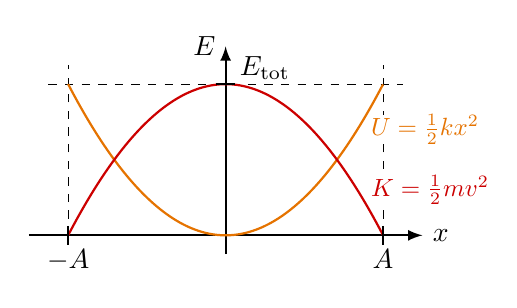
\begin{tikzpicture}
  \def\xmax{2.5}    % max x axis
  \def\ymax{2.4}    % max y axis
  \def\A{0.8*\xmax} % maximum extension
  \def\E{0.8*\ymax} % maximum total energy
  
  % AXIS
  \draw[->,thick] (0,-0.1*\ymax) -- (0,\ymax) node[left] {$E$};
  \draw[->,thick] (-\xmax,0) -- (\xmax,0) node[right] {$x$};
  \draw[dashed] (-\A,0) --++ (0,0.9*\ymax);
  \draw[dashed] ( \A,0) --++ (0,0.9*\ymax);
  \draw[dashed] (-0.9*\xmax,\E) -- (0.9*\xmax,\E);
  
  % PLOT
  \draw[xline,myorange,samples=\N,smooth,variable=\x,domain=-\A:\A]
    plot(\x,{\E/(\A*\A)*\x*\x)});
  \draw[xline,myred,samples=\N,smooth,variable=\x,domain=-\A:\A]
    plot(\x,{\E-\E/(\A*\A)*\x*\x)});
  \tick{0,\E}{180} node[above right=-2,scale=1] {$E_\text{tot}$};
  \tick{-\A,0}{90} node[below=-2,scale=1] {$-A$};
  \tick{\A,0}{90} node[below=-2,scale=1] {$A$};
  \node[myorange,right,fill=white,inner sep=0,scale=0.9] at (0.92*\A,0.7*\E) {$U = \frac{1}{2}kx^2$};
  \node[myred,right,fill=white,inner sep=0,scale=0.9] at (0.92*\A,0.3*\E) {$K = \frac{1}{2}mv^2$};
  
\end{tikzpicture}


% ENERGY vs. t
\begin{tikzpicture}
  \def\ymax{2.4} % max y axis
  \def\A{0.8*\ymax} % maximum extension
  \def\om{(2.5*360/(0.94*\xmax))} % angular frequency in degrees
  
  % AXIS
  \draw[->,thick] (0,-0.1*\ymax) -- (0,\ymax) node[left] {$E$};
  \draw[->,thick] (-0.1*\ymax,0) -- (\xmax,0) node[below] {$t$};
  \draw[dashed] (0,\A) -- (0.95*\xmax,\A);
  
  % PLOT
  \draw[xline,myorange,samples=100+\N,smooth,variable=\x,domain=0:0.94*\xmax]
    plot(\x,{\A*cos(\om*\x)^2});
  \draw[xline,myred,samples=100+\N,smooth,variable=\x,domain=0:0.94*\xmax]
    plot(\x,{\A*sin(\om*\x)^2});
  \tick{0,\A}{0} node[left=-1,scale=1] {$E_\text{tot}$};
  \tick{{360/\om},0}{90} node[below,scale=1] {$T$};
  \tick{{720/\om},0}{90} node[below,scale=1] {$2T$};
  
\end{tikzpicture}


% ENERGY vs. t - damped
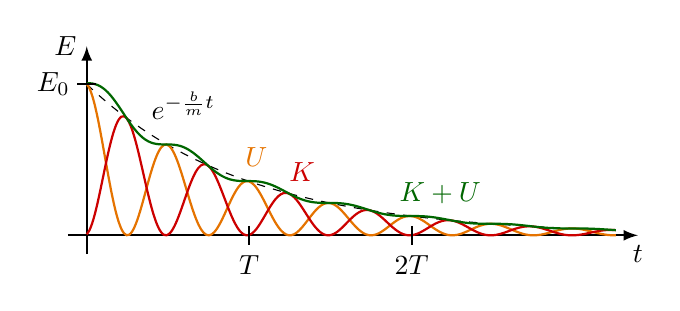
\begin{tikzpicture}
  \def\xmax{7.0} % max x axis
  \def\ymax{2.4} % max y axis
  \def\A{0.8*\ymax} % maximum extension
  \def\T{4.0}    % decay constant tau
  %\def\om{(2.5*360/(0.94*\xmax))} % angular frequency in degrees
  \def\om{(3.2*2*pi/(0.94*\xmax))} % angular frequency in radians
  \def\W{(sqrt((\om)^2-1/\T/\T))} % omega underdamped
  
  % AXIS
  \draw[->,thick] (0,-0.1*\ymax) -- (0,\ymax) node[left] {$E$};
  \draw[->,thick] (-0.1*\ymax,0) -- (\xmax,0) node[below] {$t$};
  
  % PLOT
  \draw[dashed,samples=\N,smooth,variable=\x,domain=0:0.96*\xmax]
    plot(\x,{\A*exp(-2*\x/\T)});
  \draw[xline,myorange,samples=100+\N,smooth,variable=\x,domain=0:0.96*\xmax]
    plot(\x,{\A*exp(-2*\x/\T)*cos(180/pi*\W*\x)^2});
  \draw[xline,myred,samples=100+\N,smooth,variable=\x,domain=0:0.96*\xmax]
    %plot(\x,{\A*exp(-\x/\T)*sin(180/pi*\W*\x)^2});
    plot(\x,{\A*exp(-2*\x/\T)*( 1/\T/\om*cos(180/pi*\W*\x) + \W/\om*sin(180/pi*\W*\x) )^2});
  \draw[xline,mygreen,samples=100+\N,smooth,variable=\x,domain=0:0.96*\xmax]
    plot(\x,{\A*exp(-2*\x/\T)*(cos(180/pi*\W*\x)^2 + ( 1/\T/\om*cos(180/pi*\W*\x) + \W/\om*sin(180/pi*\W*\x) )^2 )});
  \node[above right=0] at (0.1*\xmax,{\A*exp(-2*0.1*\xmax/\T)}) {$e^{-\frac{b}{m}t}$};
  \node[above right=0,myorange] at (0.27*\xmax,{\A*exp(-2*0.27*\xmax/\T)}) {$U$};
  \node[above right=0,myred] at (0.35*\xmax,{\A*exp(-2*0.35*\xmax/\T)}) {$K$};
  \node[above right=0,mygreen] at (0.55*\xmax,{\A*exp(-2*0.55*\xmax/\T)}) {$K+U$};
  \tick{0,\A}{0} node[left=-1,scale=1] {$E_0$};
  \tick{{2*pi/\W},0}{90} node[below,scale=1] {$T$};
  \tick{{4*pi/\W},0}{90} node[below,scale=1] {$2T$};
  
\end{tikzpicture}


% RESONANCE
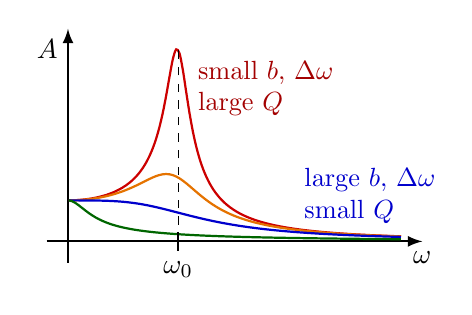
\begin{tikzpicture}
  \def\xmax{4.5}
  \def\ymax{2.7}
  \def\c{1.4}        % natural frequency
  \def\A{0.90*\ymax} % amplitude
  \def\ba{0.3}       % drag coefficient 1
  \def\bb{0.9}       % drag coefficient 2
  \def\bc{2.0}       % drag coefficient 3
  \def\bd{8.0}       % drag coefficient 4
  \coordinate (O) at (0,0);
  \coordinate (X) at (\xmax,0);
  \coordinate (Y) at (0,\ymax);
  \coordinate (C) at (\c,0);
  
  % AXIS
  \draw[->,thick]
    (-0.1*\ymax,0) -- (\xmax,0) node[below] {$\omega$};
  \draw[->,thick]
    (0,-0.1*\ymax) -- (0,\ymax) node[below left] {$A$}; %\langle{P}\rangle
  
  % PLOT
  \draw[xline,myred,samples=\N,smooth,variable=\x,domain=0.01:0.94*\xmax]
    plot(\x,{\A*\ba*\c/sqrt((\c*\c-\x*\x)^2 + (\ba*\x)^2 )});
  \draw[xline,myorange,samples=\N,smooth,variable=\x,domain=0.01:0.94*\xmax]
    plot(\x,{\A*\ba*\c/sqrt((\c*\c-\x*\x)^2 + (\bb*\x)^2 )});
  \draw[xline,myblue,samples=\N,smooth,variable=\x,domain=0.01:0.94*\xmax]
    plot(\x,{\A*\ba*\c/sqrt((\c*\c-\x*\x)^2 + (\bc*\x)^2 )});
  \draw[xline,mygreen,samples=\N,smooth,variable=\x,domain=0.01:0.94*\xmax]
    plot(\x,{\A*\ba*\c/sqrt((\c*\c-\x*\x)^2 + (\bd*\x)^2 )});
  \node[mydarkred,align=left,right,scale=0.95] at ({0.26*(\c+\xmax)},0.8*\A) {small $b$, $\Delta\omega$\\large $Q$};
  \node[myblue,align=left,above,scale=0.95] at ({0.65*(\c+\xmax)},0.3*\A*\ba/\bc) {large $b$, $\Delta\omega$\\small $Q$};
  \draw[dashed,thin] (C) --++ (0,\A);
  \tick{C}{90} node[below] {$\omega_0$};
  
  % WIDTH
  %\draw[<->,thick] ({\c/(2*\Q)*(-1+sqrt(1+4*\Q^2))},\A/2) -- ({\c/(2*\Q)*(1+sqrt(1+4*\Q^2))},\A/2);
  %\draw[width,myblue!80!black]
  %  ({\c/(2*\q)*(-1+sqrt(1+4*\q^2))},\a/2) --++ (\c/\q,0) node[midway,above] {$\Delta \omega$};
  %\draw[width,mydarkred]
  %  ({\c/sqrt(2*\Q)*(-1+sqrt(1+4*\Q^2))},\A/2) --++ {(\c/sqrt(\Q)},0)
  %  node[midway,left=0.8,above,scale=0.9] {\contour{white}{$\Delta \omega$}};
  
\end{tikzpicture}


\end{document}
